\documentclass{beamer}
\usepackage[utf8]{inputenc}
\usepackage{graphicx}
\usepackage{verbatim}  % for including code
\usepackage{tikz}
\usepackage{pgfpages} % for handout mode (if desired)
\usepackage[export]{adjustbox}
\usepackage{verbatim}

%\usepackage{utopia}


\usepackage{listings}
\lstset{%
  basicstyle=\small\ttfamily,
  language=[LaTeX]{TeX}
}
% For nicer code formatting you might consider packages like listings or minted.
%\usepackage{listings}
%\lstset{basicstyle=\tiny\ttfamily,breaklines=true}

\title{\LaTeX 101}
\subtitle{Basics for Graduate Students}
\author{Jeremy Roberts}
\institute{Kansas State University}
\date{\today}

\begin{document}

\frame{\titlepage}

%% ---------------------------------------------------------------------
%% 1. Standalone Documents
%% ---------------------------------------------------------------------

\begin{frame}[fragile]{1.a. Default, Barebones Document}
  \begin{columns}[t]
    \column{0.50\textwidth}
    %\verbatiminput{example_article.tex}
    \lstinputlisting[frame=single]{example_article.tex}

%       \textbf{Source: example\_article.tex}
%       \begin{verbatim}
% \documentclass{article}
% \begin{document}
%   Hello, world! This is a
%   barebones LaTeX article.
% \end{document}
%       \end{verbatim}
    \column{0.48\textwidth}

      %\textbf{Output:}
      % Ensure you compile example_article.tex and save its output
    %  
\includegraphics[width=\textwidth]{example_article.pdf}
      
\includegraphics[width=\textwidth,frame]{example_article.pdf}% tight frame

  \end{columns}
\end{frame}

\begin{frame}[fragile]{1.b. Lorem Ipsum Document}
  \begin{columns}[t]
    \column{0.48\textwidth}
      \textbf{Source: example\_lorem.tex}
      \begin{verbatim}
% example_lorem.tex
\documentclass{article}
\usepackage{lipsum}
\begin{document}
\lipsum[1-2]
\end{document}
      \end{verbatim}
    \column{0.48\textwidth}
      \textbf{Output:}
      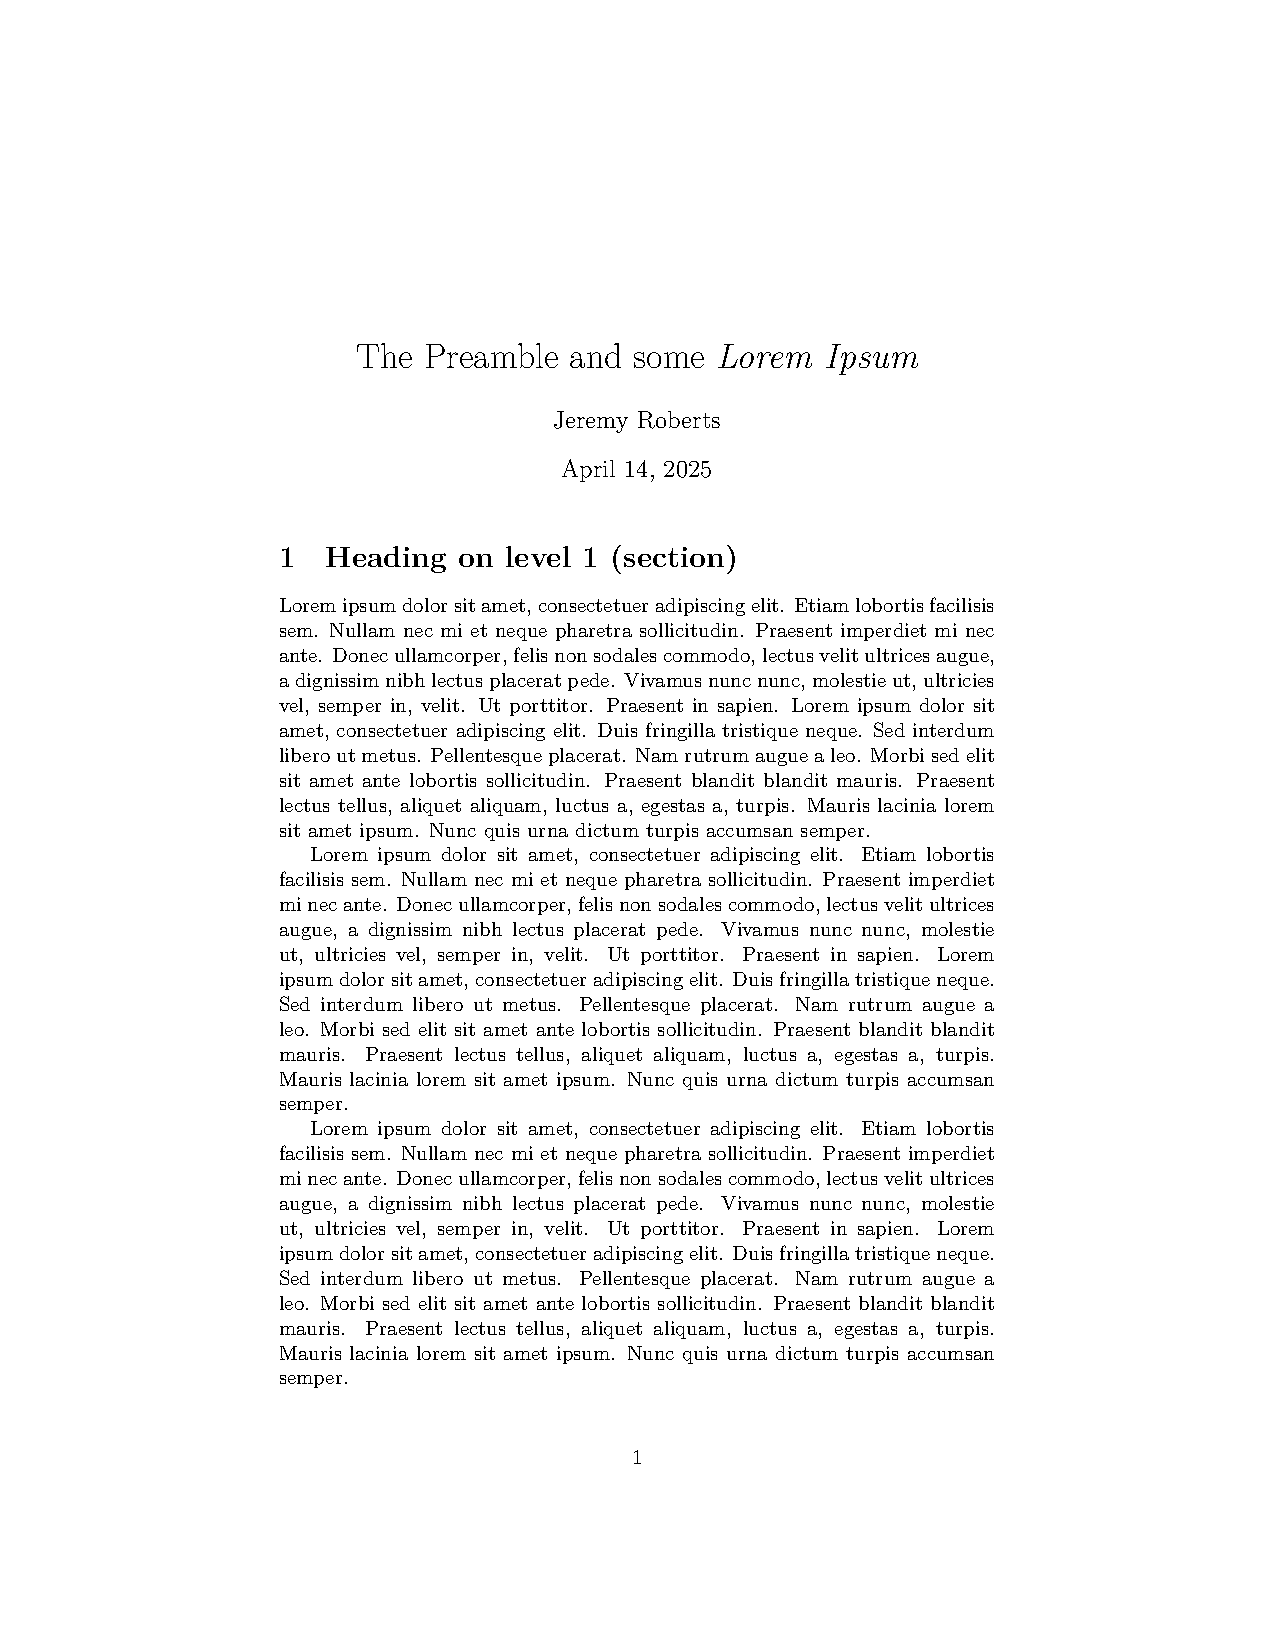
\includegraphics[width=\textwidth]{example_lorem.pdf}
  \end{columns}
\end{frame}

\begin{frame}[fragile]{1.c. Journal Template Example}
  \begin{columns}[t]
    \column{0.48\textwidth}
      \textbf{Source: example\_journal.tex}
      \begin{verbatim}
% example_journal.tex
\documentclass[twocolumn]{revtex4-2}
\begin{document}
\title{A Sample Journal Article}
\author{Author Name}
\date{\today}
\maketitle
\begin{abstract}
This is a sample abstract for a journal article.
\end{abstract}
\section{Introduction}
Sample text here.
\end{document}
      \end{verbatim}
    \column{0.48\textwidth}
      \textbf{Output:}
      \includegraphics[width=\textwidth]{example_journal_output.pdf}
  \end{columns}
\end{frame}

\begin{frame}[fragile]{1.d. Thesis Template Example}
  \begin{columns}[t]
    \column{0.48\textwidth}
      \textbf{Source: example\_thesis.tex}
      \begin{verbatim}
% example_thesis.tex
\documentclass[12pt]{report}
\begin{document}
\title{A Sample Thesis Title}
\author{Your Name}
\date{\today}
\maketitle
\chapter{Introduction}
This is the introduction.
\chapter{Literature Review}
Here is the literature review.
\end{document}
      \end{verbatim}
    \column{0.48\textwidth}
      \textbf{Output:}
      \includegraphics[width=\textwidth]{example_thesis_output.pdf}
  \end{columns}
\end{frame}

%% ---------------------------------------------------------------------
%% 2. Core Structures
%% ---------------------------------------------------------------------

\begin{frame}[fragile]{2. Core Structures: Titles, Sections, Lists, and More}
  \begin{columns}[t]
    \column{0.48\textwidth}
      \textbf{Source: example\_core\_structures.tex}
      \begin{verbatim}
% example_core_structures.tex
\documentclass{article}
\begin{document}
\title{Core Structures Example}
\author{Author}
\date{\today}
\maketitle

\section{Sections}
This is a section.

\subsection{Subsection}
This is a subsection.

\section{Lists}
\begin{itemize}
   \item First item
   \item Second item
\end{itemize}

\section{Equations}
Inline: $E=mc^2$ and display:
\[
\int_a^b f(x)\,dx
\]

\section{Tables}
\begin{tabular}{lcr}
Item & Description & Price\\
Apple & Fruit & \$1.00\\
Banana & Fruit & \$0.50\\
\end{tabular}

\section{Figures}
\begin{figure}[h]
\centering
%\includegraphics[width=0.5\textwidth]{sample-figure.jpg}
\caption{Sample figure caption.}
\end{figure}

\end{document}
      \end{verbatim}
    \column{0.48\textwidth}
      \textbf{Output:}
      \includegraphics[width=\textwidth]{example_core_structures_output.pdf}
  \end{columns}
\end{frame}

%% ---------------------------------------------------------------------
%% 3. Core Math
%% ---------------------------------------------------------------------

\begin{frame}[fragile]{3. Core Math: Symbols, Operators, Matrices, Cases}
  \begin{columns}[t]
    \column{0.48\textwidth}
      \textbf{Source: example\_core\_math.tex}
      \begin{verbatim}
% example_core_math.tex
\documentclass{article}
\usepackage{amsmath,amssymb}
\begin{document}
\section{Math Examples}

Inline math: $\alpha,\ \beta,\ \Gamma,\ \delta$.

Display math:
\[
\lim_{x\to\infty}\frac{1}{x}=0.
\]

Matrix:
\[
\begin{matrix}
a & b \\
c & d
\end{matrix}
\]

Cases:
\[
f(x)=
\begin{cases}
x^2, & x\ge0, \\
-x^2, & x<0.
\end{cases}
\]
\end{document}
      \end{verbatim}
    \column{0.48\textwidth}
      \textbf{Output:}
      \includegraphics[width=\textwidth]{example_core_math_output.pdf}
  \end{columns}
\end{frame}

%% ---------------------------------------------------------------------
%% 4. Use in Other Contexts
%% ---------------------------------------------------------------------

\begin{frame}[fragile]{4. Use in Other Contexts}
  \begin{columns}[t]
    \column{0.48\textwidth}
      \textbf{Jupyter Markdown Example (example\_jupyter.md)}
      \begin{verbatim}
<!-- example_jupyter.md -->
# Jupyter Markdown with LaTeX

Inline math: $a^2+b^2=c^2$

Displayed math:

$$
\sum_{n=1}^{\infty}\frac{1}{n^2}=\frac{\pi^2}{6}
$$
      \end{verbatim}
    \column{0.48\textwidth}
      \textbf{Notes:}\\
      In Jupyter, this Markdown renders math using MathJax.
      % You might show a screenshot of a rendered notebook.
      \includegraphics[width=\textwidth]{example_jupyter_output.pdf}
  \end{columns}

  \vspace{1ex}
  \textbf{Other:}\\
  \textbf{Word / Canvas Equations:}
  In Word or Canvas, you can often insert LaTeX‐like equations using built–in editors. For example, type
  \verb|$E=mc^2$| to render an equation.
\end{frame}

%% ---------------------------------------------------------------------
%% 5. Presentations: Beamer and Posters
%% ---------------------------------------------------------------------

% \begin{frame}[fragile]{5. Presentations: Beamer Example}
%   \begin{columns}[t]
%     \column{0.48\textwidth}
%       \textbf{Source: example\_beamer.tex}
%       \begin{verbatim}
% % example_beamer.tex
% \documentclass{beamer}
% \begin{document}
% \begin{frame}{Sample Slide}
% This is an example slide using Beamer.
% \end{frame}
% \end{document}
%       \end{verbatim}
%     \column{0.48\textwidth}
%       \textbf{Output:}
%       \includegraphics[width=\textwidth]{example_beamer_output.pdf}
%   \end{columns}
% \end{frame}

\begin{frame}[fragile]{5. Presentations: Poster Example}
  \begin{columns}[t]
    \column{0.48\textwidth}
      \textbf{Source: example\_poster.tex}
      \begin{verbatim}
% example_poster.tex
\documentclass{tikzposter}
\begin{document}
\title{Sample Poster Title}
\author{Your Name}
\maketitle
\block{Introduction}{
This is the introduction block of the poster.
}
\end{document}
      \end{verbatim}
    \column{0.48\textwidth}
      \textbf{Output:}
      \includegraphics[width=\textwidth]{example_poster_output.pdf}
  \end{columns}
\end{frame}

\end{document}
